% !TeX spellcheck = it_IT
\newpage
\section{Macchine astratte}
Alla base dei computer moderni troviamo il classico modello di Von Neumann, composto da \textbf{memoria}, che contiene dati e programmi, e \textbf{unità centrale di elaborazione}, che preleva le istruzioni, i dati necessari e le esegue una dopo l'altra. \\
Il processo eseguito da quest'ultima è il \textbf{ciclo Fetch-Decode-Execute}:
\begin{itemize}
	\item \textit{Fetch}: l'istruzione viene prelevata dalla memoria e messa nella CPU
	\item \textit{Decode}: l'istruzione viene interpretata e vengono avviati i passi necessari
	\item \textit{Data fetch}: vengono prelevati i dati necessari dalla memoria
	\item  \textit{Execute}: i passi vengono portati a termine
	\item \textit{Store}: il risultato previsto viene memorizzato
\end{itemize} 
Per implementare un \textbf{linguaggio di programmazione} che ci porti dal sorgente alla macchina abbiamo tre opzioni:
\begin{itemize}
	\item \textbf{Compilazione}: ad esempio C, che traduce direttamente il sorgente in codice macchina
	\item  \textbf{Interpretazione}: ad esempio JavaScript, si fa un'implementazione software che esegue le istruzioni del linguaggio sorgente con un processo analogo al \textit{Fetch-Decode-Execute}
	\item  \textbf{Misto}: ibrido tra i due precedenti, ad esempio Java
\end{itemize}

\begin{definition}[Macchina astratta]
	Consente l'esecuzione step-by-step dei programmi omettendo dei dettagli delle macchine reali. Rappresenta il comportamento della macchina fisica individuando:
	\begin{itemize}
		\item L'insieme delle \textbf{risorse} necessarie per l'esecuzione dei programmi
		\item L'insieme delle \textbf{istruzioni} progettate per operare con suddette risorse
	\end{itemize}
	\centering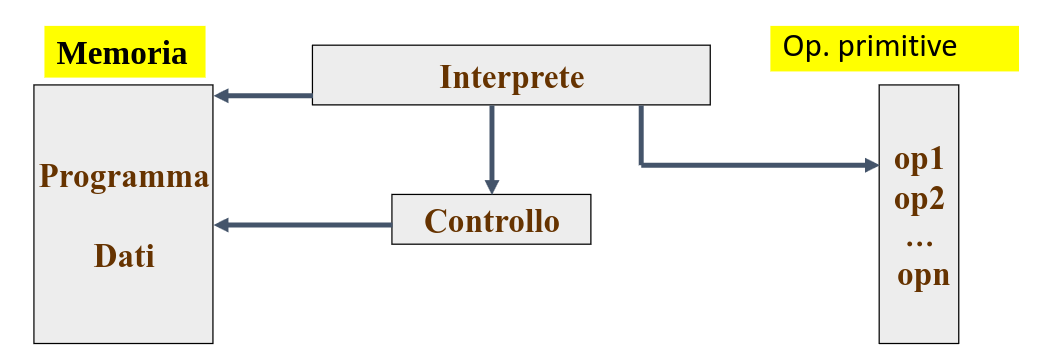
\includegraphics[width=0.98\textwidth]{macchina_astratta.png}
\end{definition}
\subsection{Interprete}
In una implementazione software, l'interprete è il \textbf{programma} che prende in ingresso il \textbf{programma da eseguire} (tipicamente l'albero di sintassi astratta del programma) e lo esegue \textbf{ispezionandone la struttura} (l'albero di sintassi) per vedere cosa deve essere fatto. 